\documentclass{beamer}

\mode<presentation>
{\usetheme{boxes}}

\usepackage{array}
\usepackage{times}
\usepackage{graphicx}
\usepackage{hyperref}
\usepackage{listings}
\usepackage{relsize}
\usepackage{ragged2e}
\usepackage[T1]{fontenc}

\lstdefinestyle{customc}{
  belowcaptionskip=1\baselineskip,
  breaklines=true,
  frame=L,
  xleftmargin=\parindent,
  language=C,
  showstringspaces=false,
  basicstyle=\footnotesize\ttfamily,
  keywordstyle=\bfseries\color{green!40!black},
  commentstyle=\itshape\color{purple!40!black},
  identifierstyle=\color{blue},
  stringstyle=\color{red},
}
\lstdefinestyle{custombash}{
  belowcaptionskip=1\baselineskip,
  breaklines=true,
  frame=L,
  xleftmargin=\parindent,
  language=bash,
  basicstyle=\footnotesize\ttfamily,
  showstringspaces=false,
  commentstyle=\itshape\color{purple!40!black},
  keywordstyle=\itshape\color{green!40!black},
  identifierstyle=\color{blue},
  stringstyle=\color{orange},
}

\usebackgroundtemplate
{
  \hbox to \paperwidth{\hfil
\includegraphics[width=4in,
      height=\paperheight]{wildcat_transparent.jpg}\hfil}
}

\title{PHYS 105 Lecture 7: Functions and Pointers}
\author{Tom McClintock \\
	Dept. of Physics\\
	University of Arizona
}
\date{\today}

\begin{document}

\begin{frame}
  \titlepage
\end{frame}

\begin{frame}
  \frametitle{Last time}
  \begin{itemize}
    \item Variable operations
    \item While loops
    \item Numerical Integration
  \end{itemize}
\end{frame}

\begin{frame}
  \frametitle{This time}
  \begin{itemize}
    \item Functions
    \item Pointers
  \end{itemize}
\end{frame}

\begin{frame}[fragile]
  \frametitle{Functions}
  A \textbf{function} is a piece of code that can be \textbf{called}.\\
  You have used functions before:
  \begin{lstlisting}[style=customc]
    printf(``stuff'');
    sin(x);
  \end{lstlisting}
  These are both examples of functions.\\
  You have also written your own function (and didn't know it!!):
  \begin{lstlisting}[style=customc]
    int main(){
      ...
    }
  \end{lstlisting}
  That's right! \textbf{main} is a function that you have 
  rewritten for all of your programs.
\end{frame}

\begin{frame}
  \frametitle{Purpose of Functions}
  To be clear, the purpose of functions are:
  \begin{itemize}
    \item Allow code to be reused
    \item Test small sections of code
    \item Organize code into independent parts with their own purposes
  \end{itemize}
  The concept of functions is what allows 
  programmers to build vastly complex programs; smaller parts can be
  connected together to do something greater.\\
  An example of this is the use of libraries.
\end{frame}

\begin{frame}[fragile]
  \frametitle{Format of functions}
  Functions have the following format:
  \begin{lstlisting}[style=customc]
    return_type function_name(input_type input_name,...)
    {
      //body
      return ...; //A return statement
    }
  \end{lstlisting}
  Functions have to have:
  \begin{itemize}
    \item A \textbf{type} for the function
    \item A \textbf{name} for the function
    \item Possibly \textbf{inputs} that have \textbf{types}
    \item A \textbf{return} statement
  \end{itemize}
\end{frame}

\begin{frame}[fragile]
  \frametitle{Using functions}
  Let's write a program that prints out all whole numbers from 
  -5 up to +5 in steps of 0.5 as well as the mathematical function:
  \begin{equation*}
    f(x) = e^{-x^2}
  \end{equation*}
  Let's have all of this printed out in columns side by side, and
  we will write $f(x)$ in its own function.\\
  \vspace{12pt}
  Note: this mathematical function is called a ``Gaussian'', also known
  as a ``normal distribution''.
\end{frame}

\begin{frame}[fragile]
  \frametitle{Example function}
  Here is what the function will look like:
  \begin{lstlisting}[style=customc]
    float f(float x); //The prototype

    int main(){
      ...
    }
    
    float f(float x){
      float y = exp(-x*x);
      return y;
    }
  \end{lstlisting}
  Note: a function needs a \textbf{prototype} before main() in order
  to use the function. Think of this just like a variable. A variable
  must be declared before it can be used. A function must be \textbf{defined}
  before it can be used, and the prototype allows this.
\end{frame}

\begin{frame}[fragile,allowframebreaks]
  \frametitle{gaussian.c}
  \lstinputlisting[style=customc]{gaussian.c}
\end{frame}

\begin{frame}[fragile]
  \frametitle{Pointers}
  Variables contain information stored \textit{somewhere} in the computer.
  \textbf{Pointers} allow us to find out where exactly this is.
  \begin{lstlisting}[style=customc]
    int j = 3; // This is an integer variable
    int* p;    // This is an integer pointer
  \end{lstlisting}
  To create a pointer to a certain type, you just add on a ``*'' 
  to the declaration.
\end{frame}

\begin{frame}[fragile]
  \frametitle{Pointer == Address}
  For our purposes, the word ``pointer'' and the word ``address''
  are synonymous. The purpose of a pointer is to point to an address
  in memory.
  \begin{lstlisting}[style=customc]
    int j = 3;
    int* p;
    
    p = &j; //p now points to the address of j
  \end{lstlisting}
  Note: adding a ``\&'' refers to a variable's address.
  You can visualize this with this helpful illustration:
  \begin{center}
    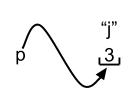
\includegraphics[width=0.5\textwidth]{pointer.pdf}
  \end{center}
\end{frame}

\begin{frame}[fragile]
  \frametitle{Dereferencing a pointer}
  Usually we aren't interested in an address, but are instead interested in
  the \textbf{information at the address}. This can be obtained by
  \textbf{dereferencing} a pointer.
  \begin{lstlisting}[style=customc]
    int j = 3;
    int* p;
    
    p = &j; //p now points to the address of j

    int k = *p; //p is dereferenced, and so k gets the value at that address
  \end{lstlisting}
  Dereferencing is obtained by adding a ``*'' in front of a pointer.
\end{frame}

\begin{frame}[fragile,allowframebreaks]
  \frametitle{pointers.c}
  Here is a short programming using pointers.
  \lstinputlisting[style=customc]{pointers.c}
\end{frame}

\begin{frame}[fragile]
  \frametitle{Pointers and functions}
  You might be asking yourself ``why are pointers useful?'' and that
  is a legitimate question. Some programming languages such as Java
  or Ruby don't give the user access to addresses of variables.
  However in C it is necessary because of how functions work.\\
  \vspace{12pt}
  Variables are ``passed by value'' to functions. In other words,
  when a variable that is an input to a function changes in the
  function, it won't change outside of the function.
\end{frame}

\begin{frame}[fragile,allowframebreaks]
  \frametitle{passbyvalue.c}
  Here is a code showing how this effect works, so that you can see
  it for yourself.
  \lstinputlisting[style=customc]{passbyvalue.c}
\end{frame}

\begin{frame}[fragile]
  \frametitle{In class assignment}
  Today there are two assignments:
  \begin{enumerate}
  \item Write a short program that contains a function that swaps the value
    of two integers passed into it.
  \item Pointers and arrays can be used in almost identical ways. 
    Write a program in which you have an array of ten integers from 0 to 9,
    and a pointer that points to the address of the first element.
    In a loop print out each element of the array as well as the current
    address the pointer points to. 
    In each loop iteration add one to the pointer:
    \begin{lstlisting}[style=customc]
      p += 1; //where p is a pointer
    \end{lstlisting}
    What do you think is happening here?
  \end{enumerate}
\end{frame}

\begin{frame}
  \frametitle{Next time}
  \begin{itemize}
    \item Graphics
    \item Random Numbers
  \end{itemize}
\end{frame}

\begin{frame}
  \frametitle{HW 4 - Trapezoid method due next week}
  The rectangle is the most basic and most inaccurate way to do
  numerical integration. The next best way is called the Trapezoid method.
  In this method, instead of finding areas of rectangles under a curve you find
  areas of trapezoids. In terms of function evaluations and the step
  size, $dx$, this has the form:
  \begin{equation*}
    A_{trap} = \frac{dx}{2}(f(x)+f(x+dx)).
  \end{equation*}
  Implement the trapezoid method, and perform the following numerical integral:
  \begin{equation*}
    \int_{-10}^{10}\sqrt{\pi}e^{-x^2}dx.
  \end{equation*}
\end{frame}

\end{document}